%%%%%%%%%%%%%%%%%%%%%%%%%%%%%%%%%%%%%%%%%
% Masters/Doctoral Thesis
% LaTeX Template
% Version 1.41 (9/9/13)
%
% This template has been downloaded from:
% http://www.latextemplates.com
%
% Original authors:
% Steven Gunn
% http://users.ecs.soton.ac.uk/srg/softwaretools/document/templates/
% and
% Sunil Patel
% http://www.sunilpatel.co.uk/thesis-template/
%
% License:
% CC BY-NC-SA 3.0 (http://creativecommons.org/licenses/by-nc-sa/3.0/)
%
% Note:
% Make sure to edit document variables in the Thesis.cls file
%
%%%%%%%%%%%%%%%%%%%%%%%%%%%%%%%%%%%%%%%%%

%----------------------------------------------------------------------------------------
%	PACKAGES AND OTHER DOCUMENT CONFIGURATIONS
%----------------------------------------------------------------------------------------

\documentclass[11pt, letter, oneside]{Thesis} % Paper size, default font size and one-sided paper

\graphicspath{{Pictures/}} % Specifies the directory where pictures are stored

\usepackage[square, numbers, comma, sort&compress]{natbib} % Use the natbib reference package - read up on this to edit the reference style; if you want text (e.g. Smith et al., 2012) for the in-text references (instead of numbers), remove 'numbers'
\hypersetup{urlcolor=blue, colorlinks=true} % Colors hyperlinks in blue - change to black if annoying
\title{\ttitle} % Defines the thesis title - don't touch this
\usepackage{amsmath}
\usepackage{amsfonts}
\usepackage{amssymb}
\usepackage{mathrsfs}
\usepackage{graphicx}
\usepackage{float}

\begin{document}

\frontmatter % Use roman page numbering style (i, ii, iii, iv...) for the pre-content pages

\setstretch{1.3} % Line spacing of 1.3

% Define the page headers using the FancyHdr package and set up for one-sided printing
\fancyhead{} % Clears all page headers and footers
\rhead{\thepage} % Sets the right side header to show the page number
\lhead{} % Clears the left side page header

\pagestyle{fancy} % Finally, use the "fancy" page style to implement the FancyHdr headers

\newcommand{\HRule}{\rule{\linewidth}{0.5mm}} % New command to make the lines in the title page

% PDF meta-data
\hypersetup{pdftitle={\ttitle}}
\hypersetup{pdfsubject=\subjectname}
\hypersetup{pdfauthor=\authornames}
\hypersetup{pdfkeywords=\keywordnames}

%----------------------------------------------------------------------------------------
%	TITLE PAGE
%----------------------------------------------------------------------------------------

\begin{titlepage}
\begin{center}

\textsc{\LARGE University of California, Merced}\\[1.5cm] % University name
\textsc{\Large Final Project Report}\\[0.5cm] % Thesis type

\HRule \\[0.4cm] % Horizontal line
\setstretch{2}{\huge  \textbf{Discrete Image Reconstruction using Parallel Beam Geometry}}\\[0.3cm] % Thesis title
\HRule \\[1.5cm] % Horizontal line
\setstretch{1.3}
\begin{minipage}{0.4\textwidth}
\begin{flushleft} \large
\emph{Authors:}\\
{Dan Hu (cs294-bu)}\\
{Lasith Adhikari (cs294-bz)}\\
{Garnet Vaz (cs294-bv)} % Author name - remove the \href bracket to remove the link
\end{flushleft}
\end{minipage}
\begin{minipage}{0.4\textwidth}
\begin{flushright} \large
\emph{Supervisor:} \\
{Dr. Phillip Colella } % Supervisor name - remove the \href bracket to remove the link
\end{flushright}
\end{minipage}\\[3cm]

\large \textit{A report submitted in fulfilment of the requirements\\ for the course of Software Engineering for Scientific Computing\\ (COMPSCI 294-73)}\\[0.3cm] % University requirement text
\textit{in the}\\[0.4cm]
Electrical Engineering \& Computer Sciences, \\ UC Berkely.\\[2cm] % Research group name and department name

{\large \today}\\[4cm] % Date
%\includegraphics{Logo} % University/department logo - uncomment to place it

\vfill
\end{center}

\end{titlepage}

%----------------------------------------------------------------------------------------
%	DECLARATION PAGE
%	Your institution may give you a different text to place here
%----------------------------------------------------------------------------------------



\clearpage % Start a new page

%----------------------------------------------------------------------------------------
%	QUOTATION PAGE
%----------------------------------------------------------------------------------------



\clearpage % Start a new page

%----------------------------------------------------------------------------------------
%	ABSTRACT PAGE
%----------------------------------------------------------------------------------------

\addtotoc{Abstract} % Add the "Abstract" page entry to the Contents

\begin{center}
\Large{\textbf{Abstract}}
\end{center}{ % Add a gap in the Contents, for aesthetics
In the context of the computerized axial tomography (CAT or CT) scan, the discrete image reconstruction using parallel beam geometry is a one of the algorithms to reconstruct the cross-sectional images of the given object. Evenly spaced set of X-ray beams are passed through an object and the intensity of the beams at input and output are measured. The aim is to reconstruct an image of the internal structure of an object from the intensity variations arising from beams passing through heterogeneous
material. This will be achieved by solving the filtered back projection formula for different readings from different angles.
}

\clearpage % Start a new page

%----------------------------------------------------------------------------------------
%	ACKNOWLEDGEMENTS
%----------------------------------------------------------------------------------------
\addtotoc{Acknowledgement}

\setstretch{1.3} % Reset the line-spacing to 1.3 for body text (if it has changed)

\begin{center}
\Large{\textbf{Acknowledgement}}
\end{center}{\addtocontents{toc}{\vspace{1em}} % Add a gap in the Contents, for aesthetics

We would like to express our special thanks of gratitude to Dr. Phillip Colella and his teaching assistance Christopher Chaplin who gave us the golden opportunity to do this wonderful project on scientific computing, which also helped us in doing a lot of research on C++ and much more.
}
\clearpage % Start a new page

%----------------------------------------------------------------------------------------
%	LIST OF CONTENTS/FIGURES/TABLES PAGES
%----------------------------------------------------------------------------------------

\pagestyle{fancy} % The page style headers have been "empty" all this time, now use the "fancy" headers as defined before to bring them back

\lhead{\emph{Contents}} % Set the left side page header to "Contents"
\tableofcontents % Write out the Table of Contents

\lhead{\emph{List of Figures}} % Set the left side page header to "List of Figures"
\listoffigures % Write out the List of Figures

\lhead{\emph{List of Tables}} % Set the left side page header to "List of Tables"
\listoftables % Write out the List of Tables

%----------------------------------------------------------------------------------------
%	ABBREVIATIONS
%----------------------------------------------------------------------------------------

\clearpage % Start a new page

%\setstretch{1.5} % Set the line spacing to 1.5, this makes the following tables easier to read
%
%\lhead{\emph{Abbreviations}} % Set the left side page header to "Abbreviations"
%\listofsymbols{ll} % Include a list of Abbreviations (a table of two columns)
%{
%\textbf{LAH} & \textbf{L}ist \textbf{A}bbreviations \textbf{H}ere \\
%%\textbf{Acronym} & \textbf{W}hat (it) \textbf{S}tands \textbf{F}or \\
%}

%----------------------------------------------------------------------------------------
%	PHYSICAL CONSTANTS/OTHER DEFINITIONS
%----------------------------------------------------------------------------------------

\clearpage % Start a new page

%\lhead{\emph{Physical Constants}} % Set the left side page header to "Physical Constants"
%
%\listofconstants{lrcl} % Include a list of Physical Constants (a four column table)
%{
%Speed of Light & $c$ & $=$ & $2.997\ 924\ 58\times10^{8}\ \mbox{ms}^{-\mbox{s}}$ (exact)\\
%% Constant Name & Symbol & = & Constant Value (with units) \\
%}

%----------------------------------------------------------------------------------------
%	SYMBOLS
%----------------------------------------------------------------------------------------

\clearpage % Start a new page

%\lhead{\emph{Symbols}} % Set the left side page header to "Symbols"
%
%\listofnomenclature{lll} % Include a list of Symbols (a three column table)
%{
%$a$ & distance & m \\
%$P$ & power & W (Js$^{-1}$) \\
%% Symbol & Name & Unit \\
%
%& & \\ % Gap to separate the Roman symbols from the Greek
%
%$\omega$ & angular frequency & rads$^{-1}$ \\
%% Symbol & Name & Unit \\
%}

%----------------------------------------------------------------------------------------
%	DEDICATION
%----------------------------------------------------------------------------------------

%\setstretch{1.3} % Return the line spacing back to 1.3
%
%\pagestyle{empty} % Page style needs to be empty for this page
%
%\dedicatory{For/Dedicated to/To my\ldots} % Dedication text
%
%\addtocontents{toc}{\vspace{2em}} % Add a gap in the Contents, for aesthetics

%----------------------------------------------------------------------------------------
%	THESIS CONTENT - CHAPTERS
%----------------------------------------------------------------------------------------

\mainmatter % Begin numeric (1,2,3...) page numbering

\pagestyle{fancy} % Return the page headers back to the "fancy" style

% Include the chapters of the thesis as separate files from the Chapters folder
% Uncomment the lines as you write the chapters

% Chapter 1

\chapter{Introduction} % Main chapter title

\label{Chapter1} % For referencing the chapter elsewhere, use \ref{Chapter1} 

\lhead{Chapter 1. \emph{Introduction}} % This is for the header on each page - perhaps a shortened title

%----------------------------------------------------------------------------------------

\section{Computerized Axial Tomography}
A computerized axial tomography (CAT or CT) scan is one of the most important non-invasive medical imaging techniques, which was developed in the early 1970's by Godfrey Hounsfield and Allen Cormack (Fig: \ref{fig:prototype})\cite{Doe:2009:Online}. X-ray CT reconstructs a cross-sectional image by computing the attenuation coefficient distribution of an object from projection data, which records the relative number of photons passing through the object.

\begin{figure}[htbp]
	\centering
		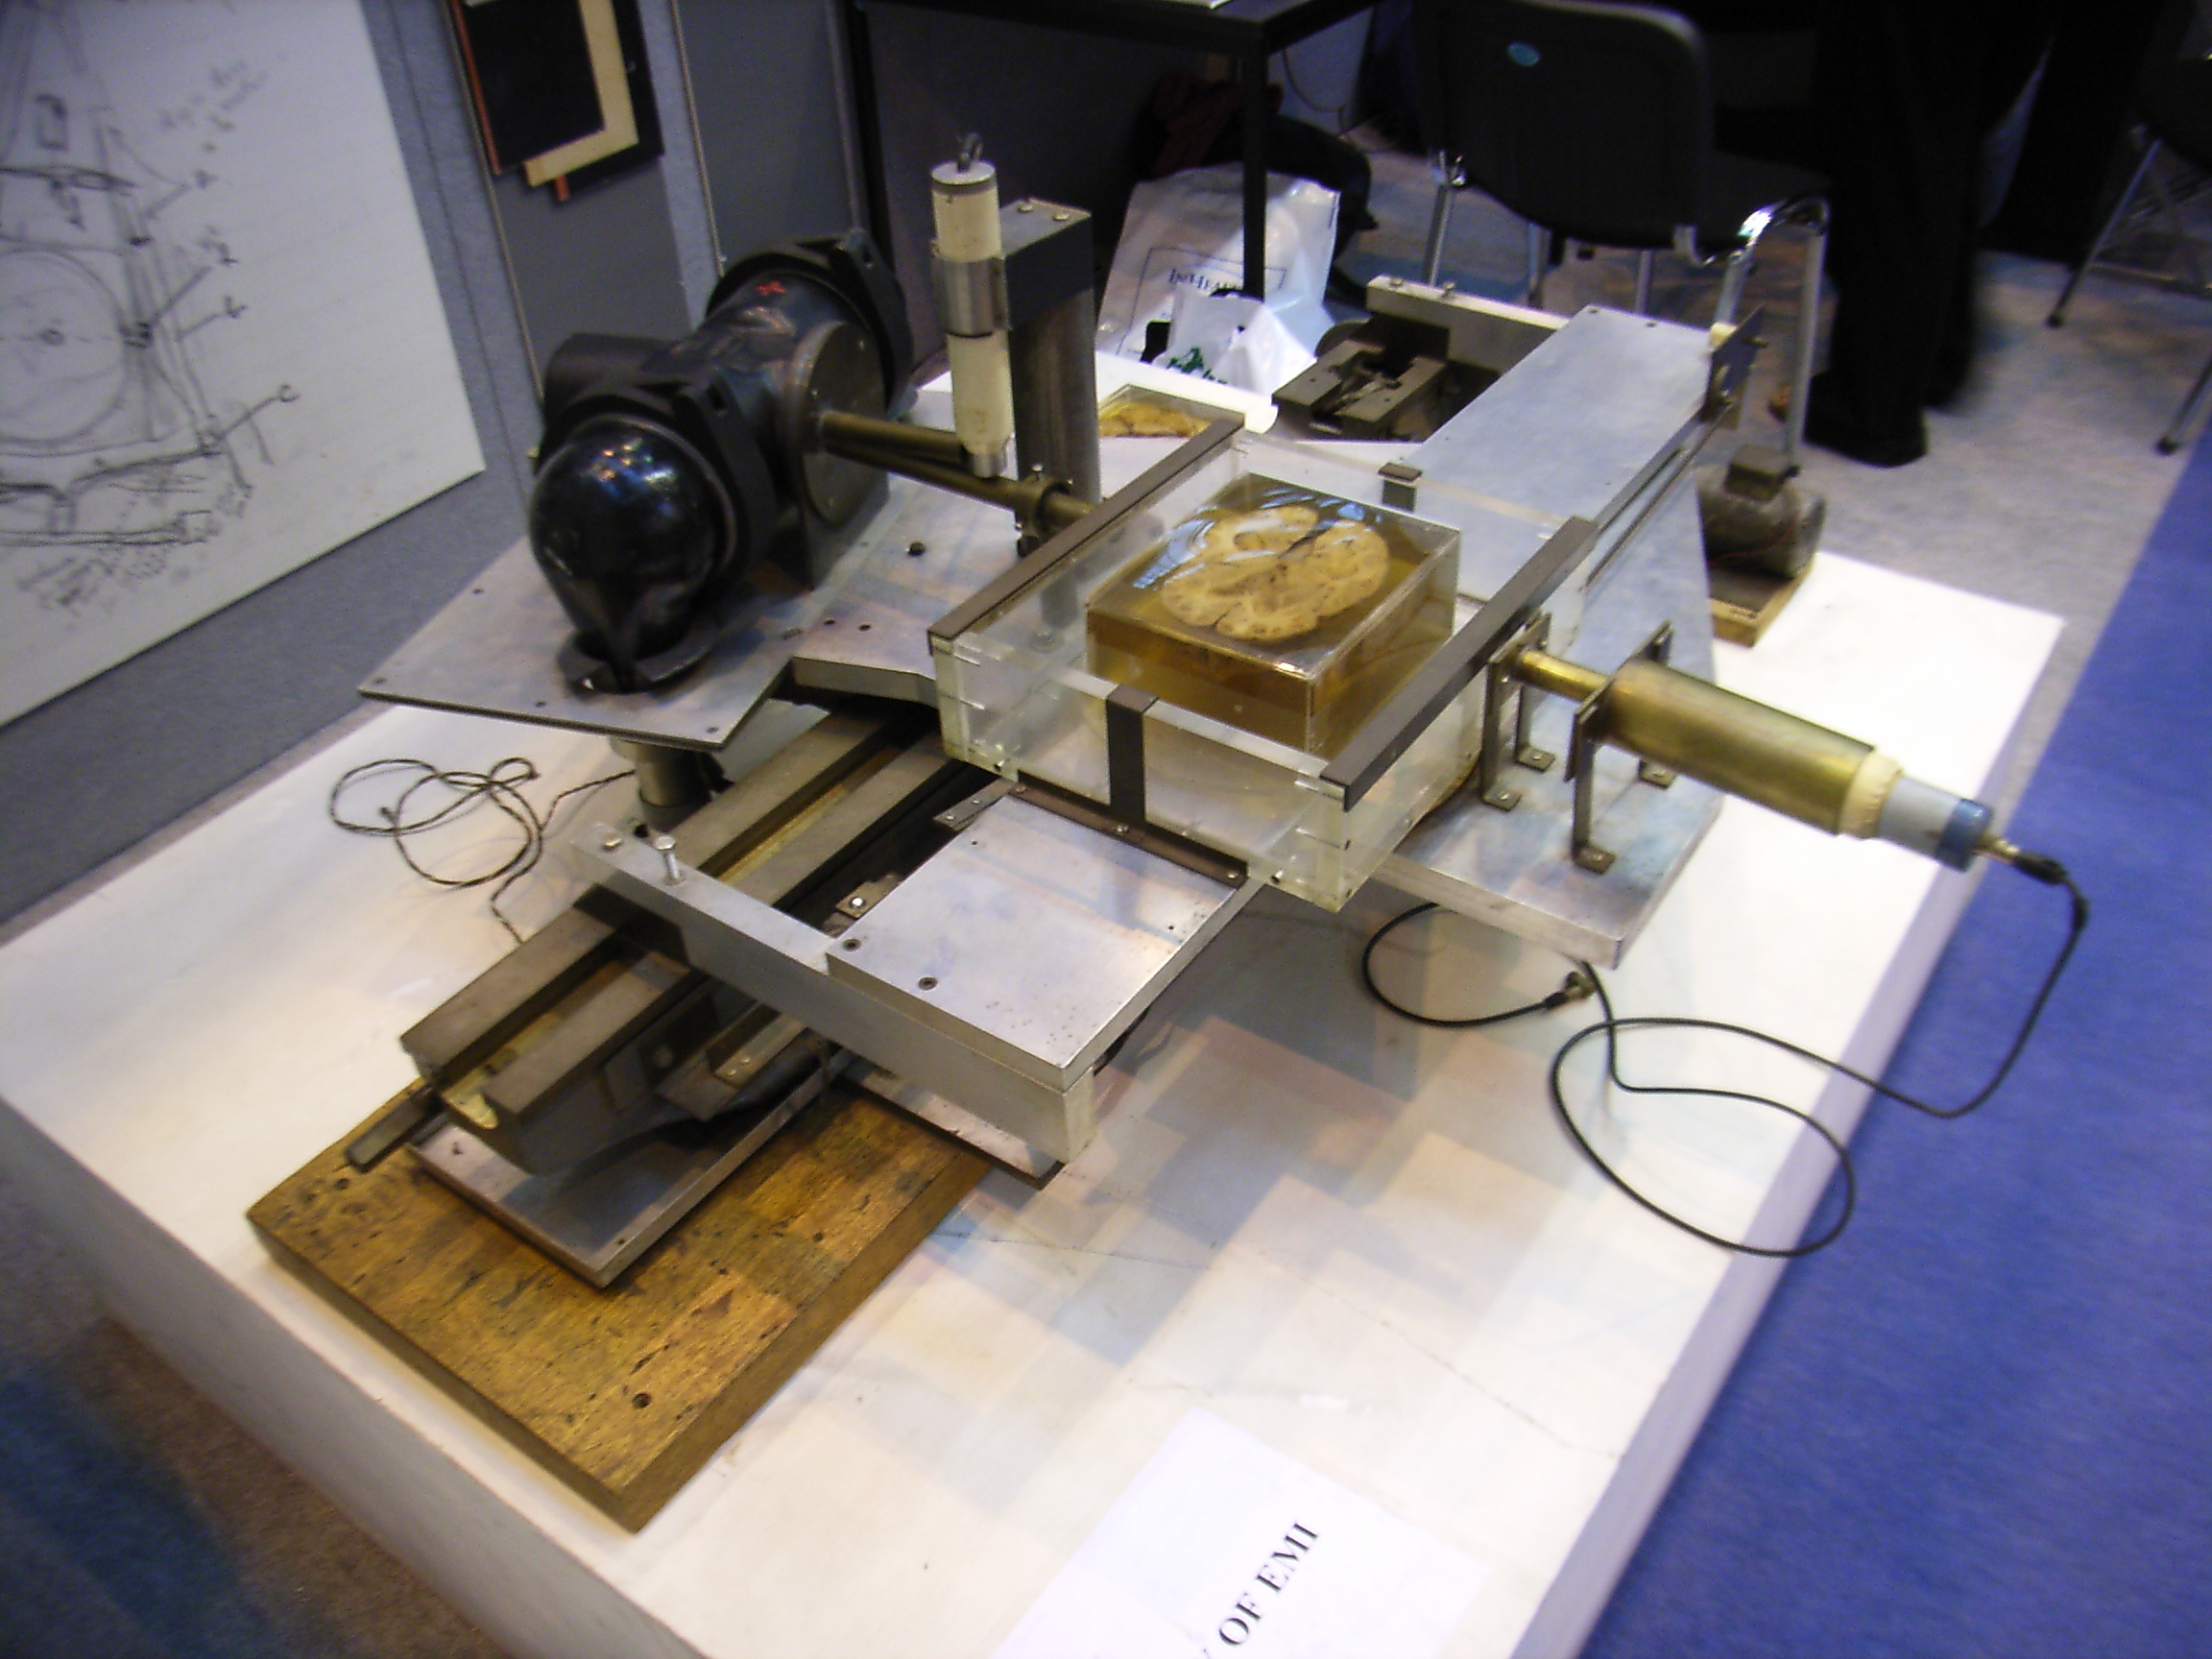
\includegraphics[width=200pt]{Figures/ct1.JPG}
	\caption[Hounsfield's prototype CT scanner]{Hounsfield's prototype CT scanner.}
	\label{fig:prototype}
\end{figure}

\section{Objective}
For the final project our team has implemented the algorithm for computerized axial tomography (CAT or CT) based on parallel beam geometry. The problem aims to solve an ill-posed inverse problem in medical imaging where X-ray beams are passed through an object and the intensity of the beams at the input and output are measured. The aim is to reconstruct an image of the internal structure of an object from the intensity variations arising from beams passing through
heterogeneous material.

Due to lack of X-ray intensity data, Shepp-Logan phantom (Fig: \ref{fig:sl}) image of the brain is used to test the reconstruction algorithm in this project. When an algorithm is applied to produce a reconstructed image of the phantom, all inaccuracies are due to the algorithm. This makes it possible to compare different algorithms in a meaningful way.   

\begin{figure}[htbp]
	\centering
		
\includegraphics[width=160pt]{Figures/Sl.png}
	\caption[Shepp-Logan Phantom]{Image of a Shepp-Logan Phantom used primarily in Tomography reconstruction.}
	\label{fig:sl}
\end{figure}


%\subsection{Figures}
%
%There will hopefully be many figures in your thesis (that should be placed in the `Figures' folder). The way to insert figures into your thesis is to use a code template like this:
%\begin{verbatim}
%\begin{figure}[htbp]
%  \centering
%    \includegraphics{Figures/Electron.pdf}
%    \rule{35em}{0.5pt}
%  \caption[An Electron]{An electron (artist's impression).}
%  \label{fig:Electron}
%\end{figure}
%\end{verbatim}
%Also look in the source file. Putting this code into the source file produces the picture of the electron that you can see in the figure below.
%
%\begin{figure}[htbp]
%	\centering
%		\includegraphics{Figures/Electron.pdf}
%		\rule{35em}{0.5pt}
%	\caption[An Electron]{An electron (artist's impression).}
%	\label{fig:Electron}
%\end{figure}


% Chapter 1
\chapter{Theory} % Main chapter title

\label{Chapter2} % For referencing the chapter elsewhere, use \ref{Chapter1} 

\lhead{Chapter 2. \emph{Theory}} % This is for the header on each page - perhaps a shortened title

%----------------------------------------------------------------------------------------

%----------------------------------------------------------------------------------------

\section{Mathematical Description}
In our study of CT-scan, we will consider a 2D slice of the
sample and assume which lies and centered on the XY-plane.

%\begin{figure}
%\begin{center}
%   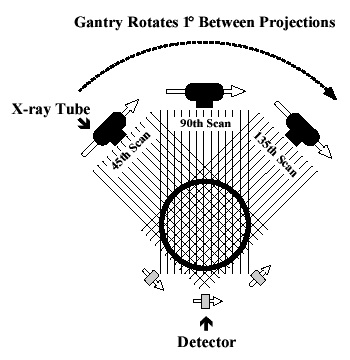
\includegraphics[width=210pt]{Figures/g1CT.jpg}
%   \caption{CT Scanner using parallel beam geometry}
%  \label{CTmodel}
%\end{center}
%\end{figure}

\begin{figure}[htbp]
	\centering
		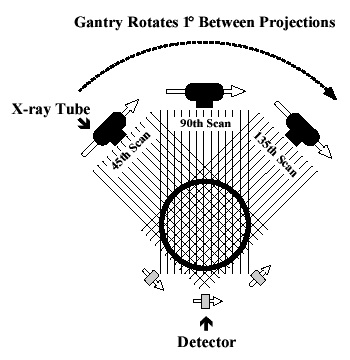
\includegraphics[width=210pt]{Figures/g1CT.jpg}
	\caption[CT scanner model]{CT Scanner using parallel beam geometry.}
	\label{fig:CTmodel}
\end{figure}


The relationship between measured intensity data ($I_0 $ :Intensity at source end, $ I_1 $ :Intensity at detector end) and attenuation-coefficients $f(x,y)$ of the material can be found by the Beer's law \cite{TimothyBook}. That is given by
\begin{equation}
ln \left( \frac{I_0}{I_1}\right) = \int_{x_0}^{x_1} f(x,y) ds.
\end{equation}
Once we parametrize the above integral along some line $l_{t,\theta}$ is called the \textit{Radon transform} and which is given by
\begin{equation}
\mathscr{R} f(t,\theta):= \int_{l_{t,\theta}} f ds=\int_{s=-\infty}^{\infty} f(tcos(\theta)-ssin(\theta),tsin(\theta)+scos(\theta))ds.
\end{equation}
Now our fundamental question is to find the function $f(x,y)$ if we know the total accumulation of the attenuation-coefficient function $f$ along every line that passes through the region. Suppose if we select some point in the plane, call it $(x_0,y_0)$, then which lies on many different lines in the plane. The first step in recovering $f(x_0, y_0)$ is to compute the average value of these line integrals averaged over all lines that pass through $(x_0, y_0)$.  This integral provides the motivation for the \textit{back-projection transform}. The back-projection of the Radon transform at $(x_0, y_0)$ is given by 

\begin{equation}\label{backproj}
\mathscr{B}\mathscr{R}f(x_0,y_0):=\dfrac{1}{\pi} \int_{\theta=0}^{\pi}\mathscr{R}f(x_0\cos(\theta)+y_0\sin(\theta),\theta) d\theta
\end{equation}
Hence, the value of the Radon transform along a given line would be the same if all of the matter there were replaced with a homogeneous sample whose attenuation coefficient was the average of the actual sample. Then the integral in equation (\ref{backproj}) is computing the average value of those averages. Thus, we can see this back-projection does not necessarily produce the exact value of $f(x_0,y_0)$. Instead it gives us an "smoothed-out" version of the attenuation coefficient.
In order to solve this problem, it is good to know the interaction between the Fourier transform and the Radon transform that is known as \textit{central slice theorem}.
\paragraph{Theorem 2.1. Central slice theorem.} For any suitable $f$ defined in the plane and all real numbers $S$ and $\theta$,
\begin{equation}\label{slice}
\mathscr{F}_2 f(S \cos(\theta), S \sin(\theta)) = \mathscr{F} (\mathscr{R} f) (S,\theta)
\end{equation}
The theorem (2.1), can be used derive new formula called the "\textit{filtered back-projection formula}" to correct the smoothing effect and recover the original function $f$.

For any suitable function $f$ and any point $(x,y)$ in the plane, by Fourier inversion theorem we can get
$$
f(x,y)=\mathscr{F}^{-1}_{2} \mathscr{F}_{2} f(x,y).
$$
By applying the definition of 2D inverse Fourier transform,
\begin{equation}\label{eq1}
f(x,y)=\dfrac{1}{4 \pi^2} \int^{\infty}_{-\infty} \int^{\infty}_{-\infty} \mathscr{F}_{2}f(X,Y) e^{i (xX+yY)} dX dY.
\end{equation}
Now change the variables such that $X=S \cos(\theta)$ and $Y=S \sin(\theta)$ where $0 \leq \theta \leq \pi \text{ and } S \in \mathbb{R}$. 
With these changes, equation (\ref{eq1}) becomes,
\begin{equation}\label{eq2}
f(x,y)=\dfrac{1}{4 \pi^2} \int^{\pi}_{0} \int^{\infty}_{-\infty} \mathscr{F}_{2}f(S\cos(\theta),S\sin(\theta)) e^{i S (x\cos(\theta)+y\sin(\theta))} |S|dS d\theta.
\end{equation}
Now with use of the central slice theorem (\ref{slice}), we can derive the "\textit{filtered back-projection formula}",
\begin{equation}\label{fback}
f(x,y) = \dfrac{1}{2} \mathscr{B} \left\lbrace  \mathscr{F}^{-1}\left[ |S|\mathscr{F} (\mathscr{R}f)(S,\theta) \right]  \right\rbrace (x,y).
\end{equation}
The filtered back-projection formula (\ref{fback}) is the fundamental basis for image reconstruction. Without the factor of $|S|$ in the formula, the Fourier transform and its inverse would cancel out and the result would be simply the back projection of the Radon transform of $f$ (see equation \ref{backproj}), which we know does not lead to recovery of $f$. Thus, the essential component in the formula is the $|S|$. Therefore we say that the Fourier transform of $\mathscr{R}f$ is filtered by multiplication by $|S|$.\\

\noindent
In practice, the above recipe for reconstructing $f$ has a problem. If the  $\mathscr{R}f$ has a component at high frequency, then that component is magnified by the factor $|S|$. This leads to exaggerate the noise by the same factor $|S|$ and which corrupts the reconstructed image. Thus, in practice, we replace $|S|$ by low-pass filter $A$.  
Then after some algebraic simplifications, function $f$ can be approximated by
\begin{equation}\label{modeqn}
f(x,y) \approx \frac{1}{2} \mathscr{B}(\mathscr{F}^{-1}A \; * \; \mathscr{R}f)(x,y),
\end{equation}
where, $(*)$ denotes the convolution of $\mathscr{F}^{-1}A$ and $\mathscr{R}f$. \\

\noindent
Here are some of the low-pass filters most commonly used in medical imaging. 

\begin{itemize}
\item[1.] The Ram-Lak filter:
\begin{eqnarray} \nonumber
A_1(\omega) = |\omega| \cdot \sqcap_{L}(\omega) = \left\{
\begin{array}{ll}
 |\omega | &\text{if } |\omega | \leq L,\\
 & \\
0 & \text{if  } |\omega | > L.\\
\end{array} \right.
\end{eqnarray}

\item[2.] The Shepp-Logan filter:
\begin{eqnarray}
A_2(\omega) &=& |\omega | \cdot \left( \frac{\sin(\pi \omega / (2L))}{\pi \omega / (2L)}\right) \cdot \sqcap_{L}(\omega) \nonumber \\
 &=& \left\{
\begin{array}{ll}
 \dfrac{2L}{\pi} |\sin(\pi \omega / (2L))| & \text{if } |\omega | \leq L,\\
 & \\
0 & \text{if  } |\omega | > L.\\
\end{array} \right. \nonumber
\end{eqnarray}

\item[3.] The Low-pass Cosine filter:
\begin{eqnarray}
A_3(\omega) &=& |\omega | \cdot \cos(\pi \omega / (2L)) \cdot \sqcap_{L}(\omega) \nonumber \\
 &=& \left\{
\begin{array}{ll}
 |\omega |\cos(\pi \omega / (2L)) & \text{if } |\omega | \leq L,\\
 & \\
0 & \text{if  } |\omega | > L.\\
\end{array} \right. \nonumber
\end{eqnarray}
\end{itemize} 



\section{Discrete Mathematical Model}
In the discrete setting, let's implement the filtered back-projection formula (\ref{modeqn}) as
$$
f(x, y) \approx   \frac{1}{2} \mathscr{B}_D \left( \mathscr{I} \left( \mathscr{F}^{-1}_{D} A \; \bar{*} \; \mathscr{R}_D f \right)\right)(x, y),
$$
where each term is described below. 
\subsection{$\mathscr{R}_Df$ is the discrete Radon transform.}
Discrete Radon transform is given by
$$
\mathscr{R}_D f_{j,k} = \mathscr{R}f (jd,k\pi/N),
$$
for $-M \leq j \leq M$ and $0 \leq k \leq (N-1)$. Suppose that there are $2\cdot M + 1$ parallel X-ray beams at each angle, $N$ different scans and beam spacing is $d$ .\\
\begin{figure}[H]
	\centering
		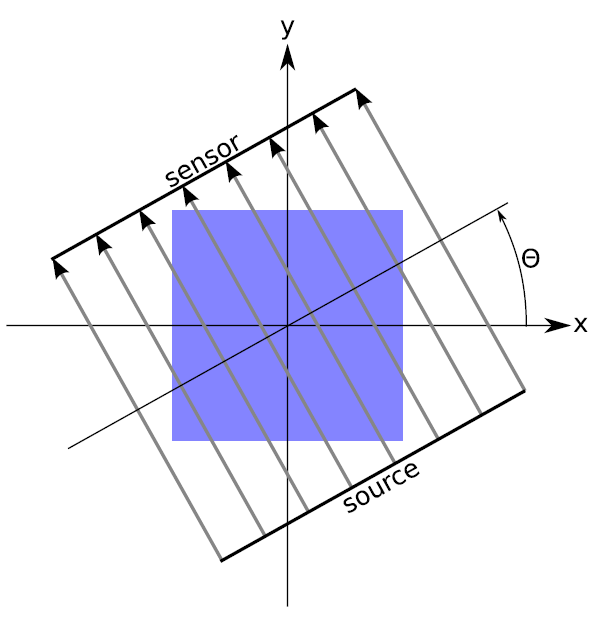
\includegraphics[width=230pt]{Figures/radon.png}
	\caption[Radon transform]{The Radon transform is a mapping from the Cartesian rectangular coordinates $(x,y)$ to a distance and an angel $(t, \theta)$, also known as polar coordinates.}
	\label{fig:radon}
\end{figure}

Finding $\mathscr{R}_D f_{j,k}$ can be thought of as computing the projection of the image along the $k$th angle and $j$th beam. The resulting projection is the sum of the intensities of the pixels along that line, i.e. a line integral. This is depicted in Figure \ref{fig:radon} \cite{Radon}.  

In order to reduce the number of calculations necessary, the maximum and minimum coordinates x or y are determined for each line (for more details see Appendix \ref{AppendixA}). 

\begin{figure}[H]
	\centering
		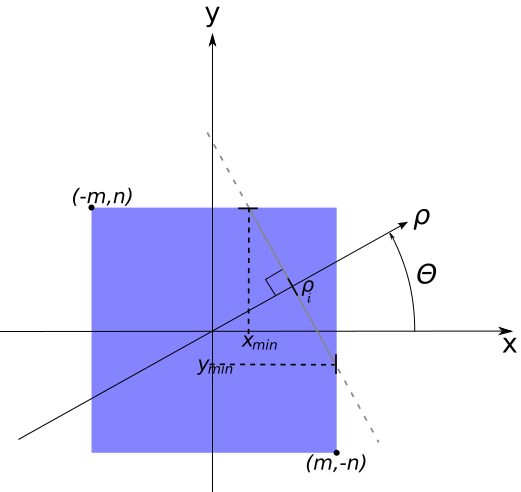
\includegraphics[width=230pt]{Figures/minmax.png}
	\caption[Maximum and minimum coordinates of x or y.]{Determining the maximum and minimum coordinates.}
	\label{fig:minmax}
\end{figure}


\subsection{$\mathscr{F}^{-1}_{D} $ is the discrete inverse Fourier transform.}
Samples for $\mathscr{F}^{-1}_{D} $ can be generated for the Shepp-Logan, Ram-Lak and low-pass cosine filters using Nyquist distance $\pi/L$ \cite{charles}.\\
Samples for discrete inverse Fourier transform of Shepp-Logan filter$(A)$ is given by
$$
(\mathscr{F}^{-1}_{D} A)_n =  \frac{4L^2}{\pi^3 (1-4n^2)}
$$
Samples for discrete inverse Fourier transform of Ram-Lak filter$(A)$ is given by
\begin{eqnarray}
\left(\mathscr{F}^{-1}A\right)_n &=& \frac{L^2}{2\pi}\left[ \frac{2\sin(\pi n)}{\pi n}-\left(\frac{\sin(\frac{\pi n}{2})}{\frac{\pi n}{2}}\right)^2 \right].\nonumber
\end{eqnarray}
If $n=0$: $(\mathscr{F}^{-1}A)(0) = L^2/2\pi$ \\
If $n$ is even : $(\mathscr{F}^{-1}A)(\frac{\pi n}{L})=0$ \\
If $n$ is odd : $(\mathscr{F}^{-1}A)(\frac{\pi n}{L})= -2L^2/(\pi^3 n^2)$\\
Samples for discrete inverse Fourier transform of low-pass cosine filter$(A)$ is given by
\begin{eqnarray}
\left(\mathscr{F}^{-1}A\right)\left(\frac{\pi n}{L}\right)&=&
\frac{2L^2}{\pi^3} \Big\lbrace  \frac{\pi \cos(\pi n)}{(1-4n^2)} -  \frac{2(4n^2+1)}{(1-4n^2)^2} \Big\rbrace \nonumber
\end{eqnarray}
The band limit $L$ in each above formulas can be found by 
$$
L = \frac{1}{2d},  \qquad \text{where } d \text{ is the beam spacing. }
$$
Fast Fourier transform also can be used to obtain the samples for each filter. 

\subsection{($\bar{*}$) denotes the discrete convolution.}
For two $N$-periodic discrete functions $g$ and $h$, the discrete convolution is defined by
$$
(g \ \bar{*} \ h)_m = \sum_{j=0}^{N-1} g_j \cdot h_{(m-j)} \text{ for each integer } m.
$$ 
\subsection{$\mathscr{I}$ is the $W$-interpolation function.}
It is defined for some discrete function $g$ as
$$
\mathscr{I}_W(g)(x) = \sum_m g(m) \cdot W\left( \frac{x}{d}-m \right) \qquad \text{for } -\infty < x < \infty. 
$$
If $W$ weighting function is square wave function,\\
i.e.
\begin{eqnarray}
\sqcap_{1/2}(x) &=& \left\{
\begin{array}{ll}
1 & \text{if } |x| < 1/2,\\
 & \\
0 & \text{if } |x| > 1/2 .\\
\end{array} \right. \nonumber
\end{eqnarray}
then it is called \textit{nearest neighbor} interpolation.\\
If $W$ is tent function,\\
i.e.
\begin{eqnarray}
\bigwedge(x) &=& \left\{
\begin{array}{ll}
1 & \text{if } |x| \leq 1,\\
 & \\
0 & \text{if } |x| > 1 .\\
\end{array} \right. \nonumber
\end{eqnarray}
then it is called \textit{linear} interpolation.  

\subsection{$\mathscr{B}_D$ is the discrete back projection.} 
For some function $h$, discrete back projection is given by
$$
\mathscr{B}_D h(x,y) = \left(\frac{1}{N}\right) \sum_{k=0}^{N-1} h(x \cos(k \pi/N)+ y \sin(k \pi/N), k \pi/N).
$$
\section{Discrete Image Reconstruction Algorithm}
By combining the all above discrete models together, we can derive the discrete image reconstruction algorithm in abstract manner \cite{TimothyBook}.\\
In the reconstruction grid, we approximate the gray scale intensity at each lattice point $(x_m, y_n)$ by
\begin{eqnarray}\label{algo}
f(x_m, y_n) &\approx & \left( \frac{1}{2}\right) \mathscr{B}_D \left( \underbrace{\mathscr{I} \left( \mathscr{F}^{-1}_{D} A \; \bar{*} \; \mathscr{R}_D f \right)}_{\mathscr{I}_0}(t,k\pi /N) \right) (x_m, y_n)  \\
&=& \left( \frac{1}{2N}\right) \sum_{k=0}^{N-1} \mathscr{I}_0  \left(x_m \cos \left(\frac{k \pi}{N}\right) + y_n \sin\left(\frac{k \pi}{N}\right), \frac{k \pi}{N}\right).\nonumber
\end{eqnarray}
% Chapter 1

\chapter{Design and Implementation} % Main chapter title

\label{Chapter3} % For referencing the chapter elsewhere, use \ref{Chapter1} 

\lhead{Chapter 3. \emph{Design and Implementation}} % This is for the header on each page - perhaps a shortened title

%----------------------------------------------------------------------------------------

\section{Architectural Design}
Class diagram of this software design is given in the figure \ref{fig:cd}. 
\begin{figure}[H]
	\centering
		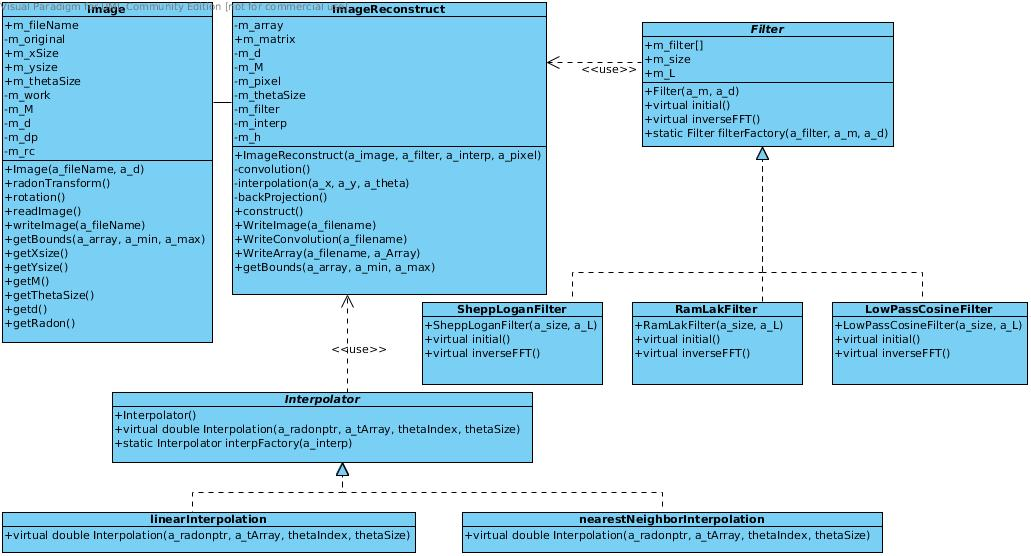
\includegraphics[width=490pt]{Figures/cd.jpg}
	\caption[Class diagram.]{Class diagram.}
	\label{fig:cd}
\end{figure}
\section{Implementation Approach}
C++ programming language in UBUNTU 12.04 platform with g++ 4.6 compiler was used to accomplish this software product. Factory design pattern was used to implement different interpolators and filters that derived from the base class. The idea of the factory pattern is to have the classes ability to create other classes without them knowing about all the possible classes that exists. 

\section{A Top Level Design of the Software}
Image reconstruction algorithm (\ref{algo}) is implemented using two main classes, i.e. \textit{Image} and \textit{ImageReconstruct} and another few minor classes for filters and interpolations. A top level design of the software used to solve this problem in the form of header files is given below.
\subsection{Image Class}
Main task of this class is to read the phantom image and compute the corresponding Radon transform. The constructor takes the file name of the image in order to read it into a RectMDArray m\_original. The double number a\_d is stored in the member data m\_d which gives the beam spacing for radon transformation. The results of the radon transformation will be updated into the member data m\_work with the type of RectMDArray which will be used in the ImageReconstruct class. This class also provides a method to write out the result of Radon transformation for testing purpose.  

\begin{verbatim}
class Image
{
public:
  Image(std::string a_fileName, double a_d);
  void radonTransform();
  void WriteImage(std::string a_fileName);
  void getBounds(RectMDArray<double>& a_array,double & a_min, double & a_max);
  int getXsize() {return m_xsize;}
  int getYsize() {return m_ysize;}
  int getM() {return m_M;}
  int getThetaSize() {return m_thetaSize;}
  double getd() {return m_d;}
  double gethalfLen() {return m_rc;}
  RectMDArray<double> getRadon() {return m_work;}
  std::string m_fileName; // Record the name of phantom image file.
 private:
  RectMDArray<double> m_original;
  RectMDArray<double> m_work;
  int m_xsize; // Record the size in the x direction of the matrix data.
  int m_ysize; // Record the sizx in the y direction of the matrix data.
  int m_thetaSize;// Record the number of rotations for the image.
  int m_M; // Record the half number of beams except zero position beam.
  double m_d; // Record the beam spacing in units
  double m_dp; // Record the beam spacing in pixels
  double m_rc; // Record the center of the image along diagonal
};
\end{verbatim}

\subsection{ImageReconstruct Class}
This class is the core of the design, which provides the major functionalities such as convolution and back projection. The member data m\_array is used to store the result of radon transformation from the Image class and after the call of convolution it will be updated to store the results of convolution. The constructor will take Image object as an input and also two integer which indicates the choices of the specific filter and interpolator. Based on the choice given by the user, the constructor will call the two static factory function of the Filter class and Interpolator class to generate the pointer to the specific derived class. The destructor of ImageReconstruct class is used to delete the filter and Interpolator pointer since these two are generated by new. Inverse FFT of the filter class are invoked inside the convolution function while interpolation functions are called inside the back projection function.   
\begin{verbatim}
class ImageReconstruct
{
public:
  RectMDArray<double> m_matrix;
  ImageReconstruct(Image & a_image, int a_filter, int a_interp, int a_pixel);
  ~ImageReconstruct();
  void construct();
  void WriteImage(std::string a_fileName);
  void WriteConvolution(std::string a_fileName);
  void WriteArray(std::string a_fileName, RectMDArray<double> a_Array);
  void getBounds(RectMDArray<double>& a_array,double & a_min, double & a_max);
 
private:
  void convolution(); // find the filtered radon transform
  void backProjection(); 
  RectMDArray<double> m_array;
  double m_d; // separation between neighbor beams
  int m_M;
  int m_thetaSize;
  int m_pixel;
  double m_h; // grid spacing in final grid
  Filter * m_filterptr;
  Interpolator * m_interpptr;
};
\end{verbatim}

\subsection{Interpolator Class}
This class is a base class which has two virtual functions that are implemented inside the derived classes shown below. In order to let user implement different Interpolation in the image reconstrcution class a factory function method is used for this base class. The factory function takes one integer indicating a specific Interpolator to create a pointer to the derived class and it returns a pointer to base class.
\begin{verbatim}
class Interpolator
{
public:
  Interpolator(){};
  virtual ~Interpolator(){};
  virtual double Interpolation(double * a_radonptr, vector<double> & a_tArray, 
      double a_t, int thetaIndex, int thetaSize) const =0;
  static Interpolator * interpFactory(int a_interp);
};  
\end{verbatim}

\paragraph{LinearInterpolator Class.}
This is a one of the derived classes of the Interpolator class, which provides the linear interpolation functionality by implementing the inherited virtual Interpolation function.  
\begin{verbatim}
class linearInterpolator:public Interpolator
{
public:
  double Interpolation(double * a_radonptr, vector<double> & a_tArray, 
  double a_t, int thetaIndex, int thetaSize) const;
};
\end{verbatim}

\paragraph{NearestNeighborInterpolator Class.}
This is the other derived class of the Interpolator class, which provides the nearest neighbor interpolation functionality by implementing the inherited virtual Interpolation function.  
\begin{verbatim}
class nearestNeighborInterpolator: public Interpolator
{
public:
  double Interpolation(double * a_radonptr, vector<double> & a_tArray, double a_t, int thetaIndex, int thetaSize) const;
};
\end{verbatim}

\subsection{Filter Class}
This class is a base class which has three virtual functions that are implemented inside the derived classes shown below. The factory function filterFactory is also used here.
\begin{verbatim}
class Filter
{
public:
  Filter(int a_m, double a_d){ m_size=2*a_m; m_L = 1.0/(2.*a_d); m_filter.resize(2*m_size+1); } 
  virtual ~Filter(){};
  virtual void inverseFFT()=0; 
  virtual void initial() = 0;
  static Filter* filterFactory(int a_filter, int a_m, double a_d);
  vector<double> m_filter;
  int m_size; // the size of filter = 2*m_size +1 = 4*a_size +1
  int m_L;
};  
\end{verbatim}

\paragraph{SheppLoganFilter Class.}
This is a one of the derived classes of the Filter class, which provides the Shepp-Logan filter functionality by implementing the inherited virtual inversFFT function.  
\begin{verbatim}
class SheppLoganFilter: public Filter
{
public:
  SheppLoganFilter(int a_size, double a_L): Filter(a_size, a_L) { }; 
  void inverseFFT(){};
  void initial(){};
};
\end{verbatim}

\paragraph{RamLakFilter Class.}
This is a another derived class of the Filter class, which provides the Ram-Lak filter functionality by implementing the inherited virtual inversFFT function.  
\begin{verbatim}
class RamLakFilter: public Filter
{
public:
  RamLakFilter(int a_size, double a_L): Filter(a_size, a_L) { }; 
 void inverseFFT(){};
 void initial(){};
};
\end{verbatim}

\paragraph{LowPassCosineFilter Class.}
This is also a derived classes of the Filter class, which provides the low-pass cosine filter functionality by implementing the inherited virtual inversFFT function.  
\begin{verbatim}
class LowPassCosineFilter: public Filter
{
public:
  LowPassCosineFilter(int a_size, double a_d): Filter(a_size, a_d) { };
  void inverseFFT(){};
  void initial(){};
};
\end{verbatim}





\chapter{Results} % Main chapter title

\label{Chapter4} % For referencing the chapter elsewhere, use \ref{Chapter1} 

\lhead{Chapter 4. \emph{Results}} % This is for the header on each page - perhaps a shortened title

%----------------------------------------------------------------------------------------
\setstretch{1}
\section{System Inputs}
Using the Figure \ref{fig:phantom} as the input phantom image, all the resulted reconstructed images were obtained with the image reconstruction algorithm as described in the chapter 2.  

\begin{figure}[H]
	\centering
		
\includegraphics[width=150pt]{Figures/Sl.png}
	\caption[Input Phantom Image.]{Shepp-Logan Phantom Image.}
	\label{fig:phantom}
\end{figure}
%----------------------------------------------------------------------------------------

This software allows user to select the size of the image to be constructed in the run time. For a instance, 

\begin{verbatim}
Please input the image file number to be constructed: 
 1 - Shepp_Logan image with size 256 x 256
 2 - Shepp_Logan image with size 200 x 200
 3 - Shepp_Logan image with size 100 x 100
Your choice: 1
\end{verbatim}
As a system constrained, we always use square, even size gray-scale  PGM ASCII image format. 

Then the user has to input the required X-ray beam spacing that will be used to perform the radon transform. As a user guidance, this software system will provide minimum beam spacing if the user really wants to use the maximum number of beams for the reconstruction process.

As the next inputs, user has to select the type of the filter and the interpolation method that he/she wants to apply on the image. For a instance, 
\begin{verbatim}
Please input the type of the Filter: 
 1 : Shepp-Logan filter
 2 : Ram-Lak filter 
 3 : Low-pass cosine filter 
Your choice: 1
 
Please input the type of the Interporlator: 
 1 : Linear Interpolator
 2 : Nearest neighbor Interpolator 
Your choice: 1
\end{verbatim}

After that the system will generate and store the corresponding reconstructed image along with the Radon transform image and the convolution image inside the main folder. User can compare the output image with the original image stored inside the Phantom folder.   

\section{System Outputs}
According to the above input parameters, we can see that there are different possible combinations that user can use while executing the system. But here we are going to consider only few important test cases. 

\subsection{Test case 1:}
\begin{itemize}
\item Image size: $256 \times 256$
\item Beam spacing: 0.005 (i.e 363 beams)
\item Filter: Shepp-Logan
\item Interpolator:  Linear 
\end{itemize}

\paragraph{Radon Transformation}
The output of the radon transformation for the test case 1 is shown in the Figure \ref{fig:radont1}.  
\begin{figure}[H]
	\centering
		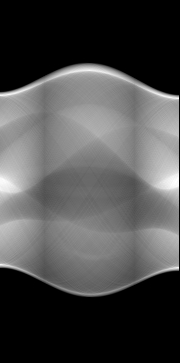
\includegraphics[width=80pt]{Figures/RadonTransform256.jpg}
	\caption[Radon transform of test case 1.]{Radon transform of test case 1.}
	\label{fig:radont1}
\end{figure}

\paragraph{Convolution}
The output of the convolution (i.e. filtered Radon transformation) for the test case 1 is shown in the Figure \ref{fig:cont1}.  
\begin{figure}[H]
	\centering
		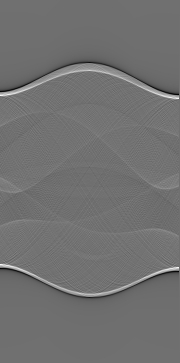
\includegraphics[width=80pt]{Figures/Convolution256.jpg}
	\caption[Convolution of test case 1.]{Convolution of test case 1.}
	\label{fig:cont1}
\end{figure}

\paragraph{Back projection Transformation}
Corresponding reconstructed image is given by the Figure \ref{fig:t1}.  
\begin{figure}[H]
	\centering
		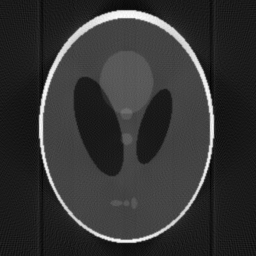
\includegraphics[width=150pt]{Figures/ReconstructedImage256.jpg}
	\caption[Test case 1 image.]{Test case1: Reconstructed phantom.}
	\label{fig:t1}
\end{figure}

The error related to the above reconstruction is given by the Figure \ref{fig:error}.  
\begin{figure}[H]
	\centering
		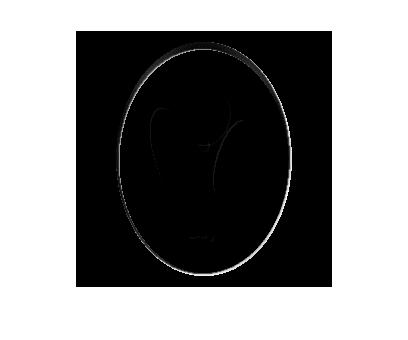
\includegraphics[width=230pt]{Figures/error.jpg}
	\caption[Reconstruction error image.]{Error of test case 1.}
	\label{fig:error}
\end{figure}

According to the error image \ref{fig:error}, we can conclude that the most of intensity errors occurred only near the edges of the phantom image.




\subsection{Test case 2:}
\begin{itemize}
\item Image size: $256 \times 256$
\item Beam spacing: 0.02 (i.e 121 beams)
\item Filter: Shepp-Logan
\item Interpolator:  Linear 
\end{itemize}
Corresponding reconstructed image is given by the Figure \ref{fig:t2}.  
\begin{figure}[H]
	\centering
		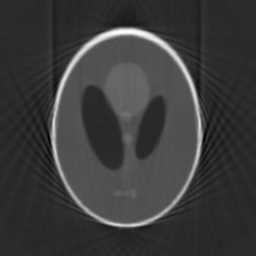
\includegraphics[width=150pt]{Figures/ReconstructedImage256t2.jpg}
	\caption[Test case 2 image.]{Test case2: Reconstructed phantom.}
	\label{fig:t2}
\end{figure}
According to the output image \ref{fig:t2}, we can see that the image become little blurred and distorted with respect to the Figure \ref{fig:t1}. This is because, for test case 2, we only used one third of beams compared to the test case 1. But this process is much faster than test case 1 process. 

Similar to this test cases, user can reconstruct image using different interpolators and filters provide by this system. 

\section{Performance Analysis }
From our experience the linear interpolator with the Shepp-logan filter or Low pass cosine filter will give the best result of the image reconstruction. Therefore in the following we will analyze the result using the linear interpolator and Shepp-logan filter setting for the code.

\begin{table}[htp]
\centering
\begin{tabular}{|c |c| c |c |}
 \hline
 \multicolumn{2}{|c|}{[1] main.cpp }& \multicolumn{2}{|c|}{ time = 14.1911 } \\
 \hline
subroutine & Time Percentage & total time & loops \\
 \hline
[6] Radon Transformation & $0.9\%$ & 0.1225 & 1\\
  \hline
[2] Image Reconstruction &  $70.1\%$ & 9.9471 & 1\\
 \hline
  \multicolumn{2}{|c|}{[2] Image Reconstuction }& \multicolumn{2}{|c|}{time = 9.9471} \\
 \hline
subroutine & Time Percentage & total time & loops \\
 \hline
[3] Back Projection & $99.8\%$ & 9.9236 & 1\\
  \hline
[7] Convolution &  $0.2\%$ & 0.0235 & 1\\
 \hline
   \multicolumn{2}{|c|}{[3] Back Projection  }& \multicolumn{2}{|c|}{time = 14.0130} \\
 \hline
 subroutine & Time Percentage & total time & loops \\
 \hline
[4] Summation over $\theta$ & $96.2\%$ & 9.5455 & 65536\\
  \hline
[8] Linear Index &  $0.0\%$ & 0.001 & 65536\\
 \hline
   \multicolumn{2}{|c|}{[4] Summation over $\theta$  }& \multicolumn{2}{|c|}{time = 9.5455} \\
 \hline
 subroutine & Time Percentage & total time & loops \\
 \hline
[5] Linear Interpolation & $92.1\%$ & 8.7874 & 11796480\\
  \hline
[8] Calculation of t &  $6.571\%$ & 0.6270 & 11796480\\
 \hline
    \multicolumn{2}{|c|}{[5] Linear Interpolation  }& \multicolumn{2}{|c|}{time = 8.7874} \\
 \hline
 subroutine & Time Percentage & total time$^*$ & loops \\
 \hline
[5] tent & $30.4\%$ & 2.671 & 4282122240\\
  \hline
[8] Linear Index &  $45.3\%$ & 3.984 & 4282122240\\
 \hline
\end{tabular}
\caption{Time table for main.exe for image of 256 x 256 and the beam spacing is chosen as d=0.007. Shepp-logan filter and linear interpolator are used in this run. Notice that in the subroutine of Linear Interpolator only the precentage is measured by Timer. The time inside this subroutine is calculated from the precentage of total time.}\label{table1}
\end{table}

The results from timer are in shown in the time Table.\ref{table1}. From this figure it is easy to notice that most of the time is cost in the back projection part. Because there are three loops inside the back projection and the interpolation is called 11796480 times in order to do the back projection for output figure with 256x256 pixels. Most of the time are cost inside these loops. In order to optimize the code we already used the linear index to access the element of all the RectMDArray objects. It is shown in the table that linear index has the same order of time consume with other flop operation. All function asr actually made in line since we used -o3 option in the compiler and we inline all possible member functions inside interpolator class. Therefore the only way to optimize the code is to parallelize the back projection because the back projection are independent with each other and the loops inside it is most time consuming.

The timer class has a bug in it which it could allow use the timer inside another timer and by including it inside the inner loops of interpolator class it really slow down the code into 100 seconds. Because there are too many loops here timer in the most inside loop will definitely slow down the code. Therefore in the most inner subroutine we use the timer to calculate the percentage of each function but calculate the real time by multiply the percentage with the total time of the parent subroutine.

%\input{Chapters/Chapter5}
%\input{Chapters/Chapter6}
%\input{Chapters/Chapter7}

%----------------------------------------------------------------------------------------
%	THESIS CONTENT - APPENDICES
%----------------------------------------------------------------------------------------

\addtocontents{toc}{\vspace{2em}} % Add a gap in the Contents, for aesthetics

\appendix % Cue to tell LaTeX that the following 'chapters' are Appendices

% Include the appendices of the thesis as separate files from the Appendices folder
% Uncomment the lines as you write the Appendices

% Appendix A

\chapter{Calculating Coordinates for Line Integrals of Radon Transform} % Main appendix title

\label{AppendixA} % For referencing this appendix elsewhere, use \ref{AppendixA}

\lhead{Appendix A. \emph{Radon transform}} % This is for the header on each page - perhaps a shortened title

These minimum and maximum coordinates are calculated depends on in which of the four areas (see Figure \ref{fig:areas} ) $\theta$ resides. Because when the summation line has an absolute inclination of more than 1 will cause some pixels to be skipped.

\begin{figure}[H]
	\centering
		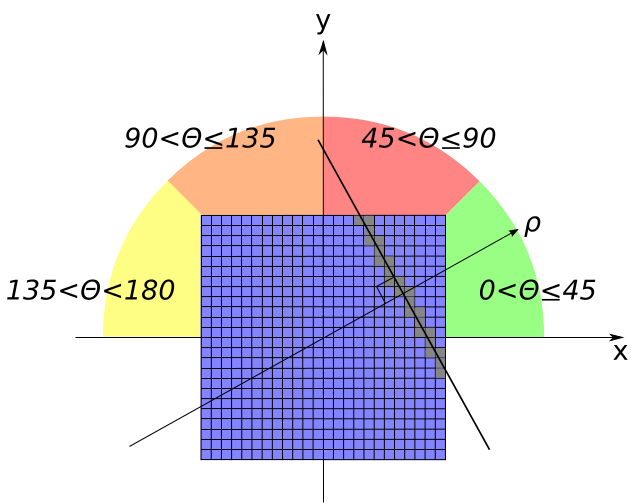
\includegraphics[width=230pt]{Figures/regions.png}
	\caption[Minimum and maximum coordinates in each region.]{Determining the maximum and minimum coordinates based on $\theta$ region.}
	\label{fig:areas}
\end{figure}


The formulas used to calculate the minimum and maximum of the variable depending on the angle $\theta$ are given below. Where $m$ is half the width of the image and $n$ is half the height of the image, $a$ is inclination, $b$ is 	the intersection with the $y$-axis and the $t_{max}$ is the size of the diagonal of the image , i.e. $t_{max}\lceil \sqrt{(2m)^2 + (2n)^2}\rceil$.
\begin{eqnarray}
0 < \theta \leq 45: \qquad  x &=& \frac{y-b}{a} \nonumber \\
	y_{min} &=& max(-n, am + b) \nonumber \\
	y_{max} &=& min(n, -am + b) \nonumber 
\end{eqnarray}

\begin{eqnarray}
45 < \theta \leq 90: \qquad  y &=& ax+b \nonumber \\
	y_{min} &=& max(-m, \frac{n-b}{a}) \nonumber \\
	y_{max} &=& min(m, \frac{-n-b}{a}) \nonumber 
\end{eqnarray}

\begin{eqnarray}
90 < \theta \leq 135: \qquad  y &=& ax+b \nonumber \\
	y_{min} &=& max(-m, \frac{-n-b}{a}) \nonumber \\
	y_{max} &=& min(m, \frac{n-b}{a}) \nonumber 
\end{eqnarray}

\begin{eqnarray}
135 < \theta \leq 180: \qquad  x &=& \frac{y-b}{a} \nonumber \\
	y_{min} &=& max(-n, -am + b) \nonumber \\
	y_{max} &=& min(n, am + b) \nonumber 
\end{eqnarray}

\begin{eqnarray}
\theta = 180: \qquad  t &=& x+ \lceil \frac{t_{max}-2m}{2} \rceil \nonumber \\
	y &=& [-m, m] \nonumber
\end{eqnarray}

%\input{Appendices/AppendixB}
%\input{Appendices/AppendixC}

\addtocontents{toc}{\vspace{2em}} % Add a gap in the Contents, for aesthetics

\backmatter

%----------------------------------------------------------------------------------------
%	BIBLIOGRAPHY
%----------------------------------------------------------------------------------------

\label{Bibliography}

\lhead{\emph{Bibliography}} % Change the page header to say "Bibliography"

\bibliographystyle{unsrtnat} % Use the "unsrtnat" BibTeX style for formatting the Bibliography

\bibliography{Bibliography} % The references (bibliography) information are stored in the file named "Bibliography.bib"

\end{document}